\documentclass{article}
\usepackage[utf8]{inputenc}
\usepackage[spanish]{babel}
\usepackage{listings}
\usepackage{graphicx}
\graphicspath{ {images/} }
\usepackage{cite}

\begin{document}

\begin{titlepage}
    \begin{center}
        \vspace*{1cm}
            
        \Huge
        \textbf{Proyecto juego }
            
        \vspace{0.5cm}
        \LARGE
        
            
        \vspace{1.5cm}
            
        \textbf{Diego Fernando Urbano Palma}
        \textbf{Sebastian Giraldo Gomez}
            
        \vfill
            
        \vspace{0.8cm}
            
        \Large
        Despartamento de Ingeniería Electrónica y Telecomunicaciones\\
        Universidad de Antioquia\\
        Medellín\\
        Marzo de 2021
            
    \end{center}
\end{titlepage}

\tableofcontents
\newpage
\section{ introduccion}\label{intro}
C++ es un lenguaje de programación diseñado en 1979 por Bjarne Stroustrup. La intención de su creación fue extender al lenguaje de programación C mecanismos que permiten la manipulación de objetos. En ese sentido, desde el punto de vista de los lenguajes orientados a objetos, C++ es un lenguaje híbrido.
Este proyecto tiene como finalidad crear un juego con el lenguaje C++ que abarca lo visto en el curso de informatica 2 de la Universidad de Antioquia.

\section{defensa de cañon } \label{contenido}
en el presente proyecto, se quiere recrear un juego bidimensional, fácil de entender o de curva de aprendizaje baja, llevado por niveles donde se tiene que aguantar oleadas hasta llegar el final del nivel.

La primicia del juego es de un cañón el cual debe defender su fortaleza de enemigos que van apareciendo por oleadas el cañón solo puede pistara en aun dirección por lo cual debe mover por el perímetro del muro que protege.
 



\begin{figure}[h]
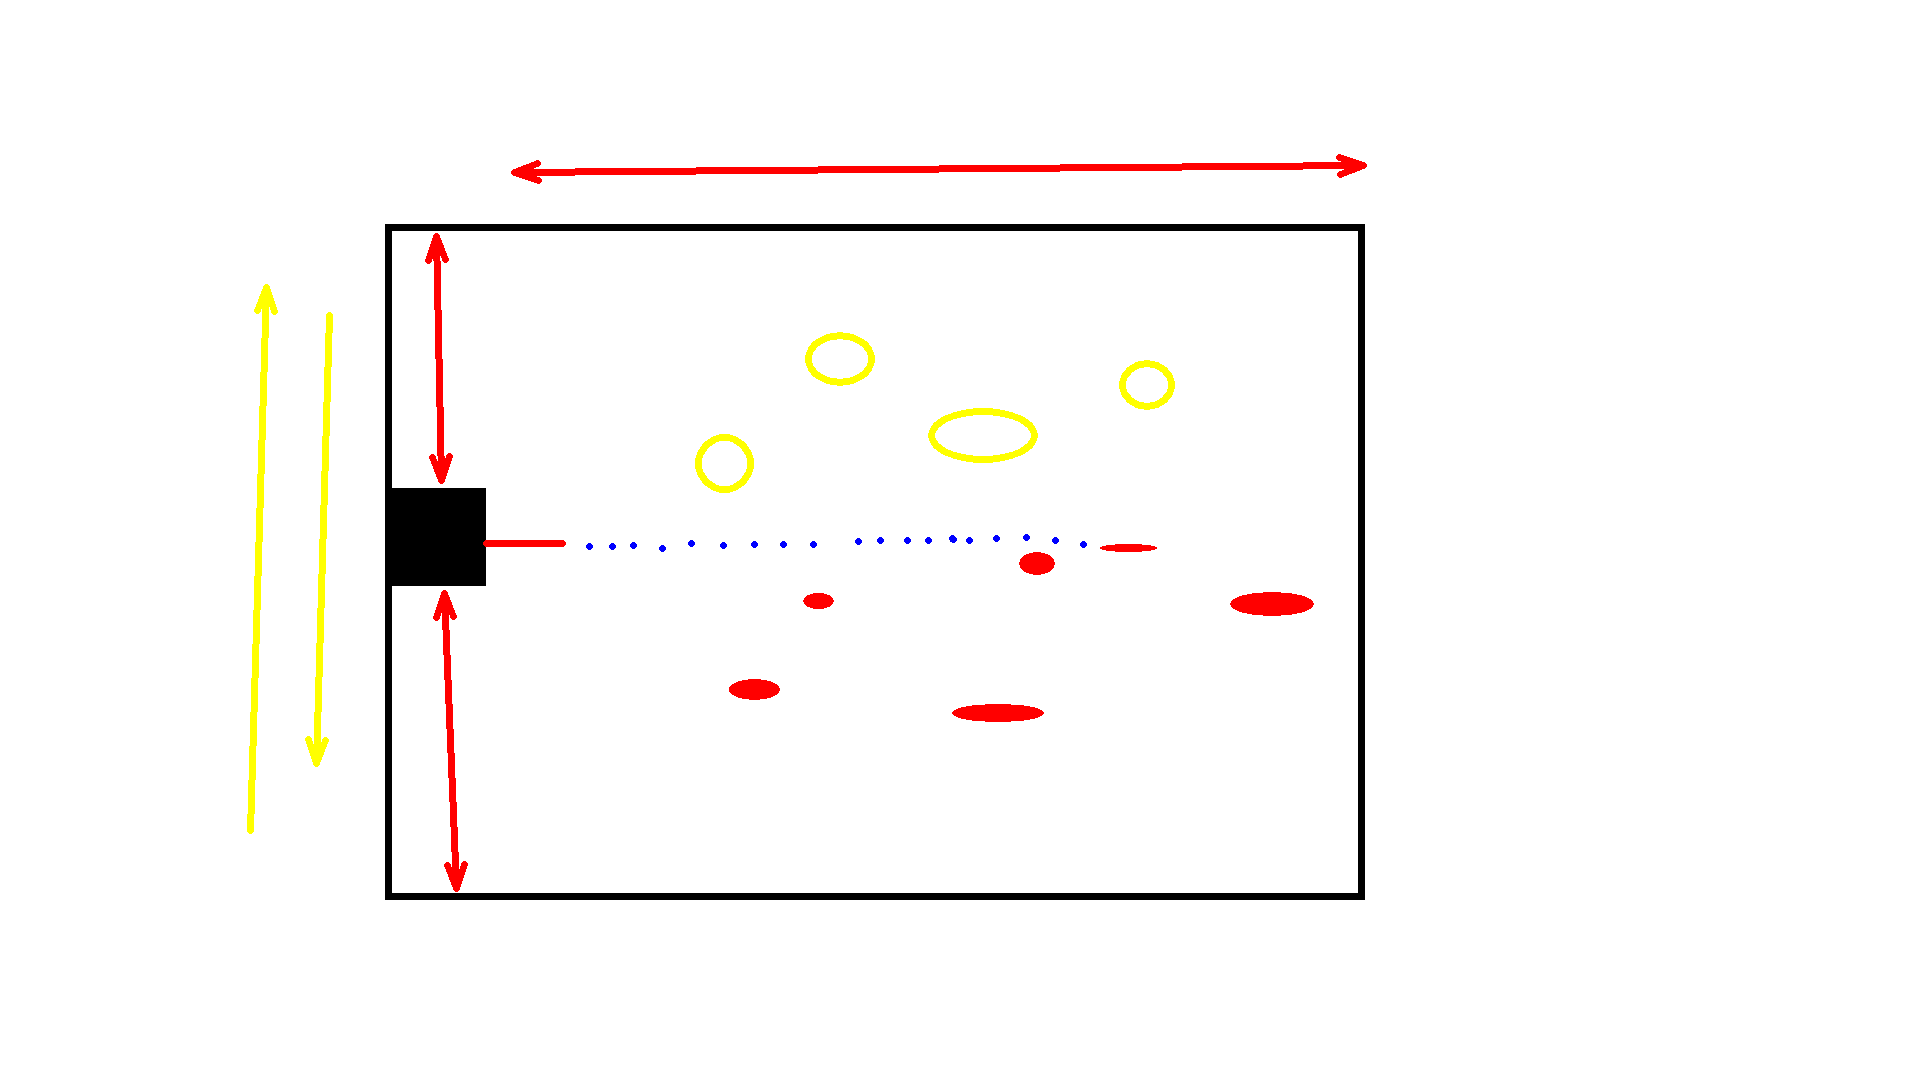
\includegraphics[width=12cm]{cañon.png}
\centering
\caption{Imagen ilustrativa del juego}
\label{fig:cpplogo}
\end{figure}


\bibliographystyle{IEEEtran}


\end{document}
